\chapter{Statistical Learning}
\hl{reference statistical learning (voir mas1)}

This section do not cover all the formulas talk in the book since we already seen it in \emph{Modèle Linéaire en actuariat}. This section talk more about the analysis of some statistical model.

\section{Statistical Learning}

\paragraph{Prediction}
\begin{align*}
    \esp{Y - \hat{Y}} &= \esp{f(x) + \varepsilon - \hat{f}(x)}^2 \\
                      &= [f(x) - \hat{f}(x)]^2 + \variance{\varepsilon} \\
                      &= (\text{Réductible}) + (\text{Irreductible)}
\end{align*}

\paragraph{Inference}
We are often interested in understanding the way that Y is affected as $X_1,...,X_p$ is changing. Inference mean that we want to understand the relationship between X and Y, or more specifically, to understand how Y changes as a function of $X_1,...,X_p$ 
\begin{itemize}
    \item Which predictors are associated with the response?
    \item What is the relationship between the response and each predictor?
    \item Can the relationship between Y and each predictor be adequately summarized using a linear equation, or is the relationship more compli cated?
\end{itemize}

\subsection{How Do We Estimate f?}
\paragraph{Parametric Methods}
Parametric methods involve a two-step model-based approach.

\begin{enumerate}
    \item  First, we make an assumption about the functional form, or shape, of f. For example, one very simple assumption is that f is linear in X: \[ f(X) = \beta_0 + \beta_1 X_1 + ... + \beta_p X_p \]
    \item  After a model has been selected, we need a procedure that uses the training data to fit or train the model.enumarate
\end{enumerate}

The potential disadvantage of a parametric approach is that the model we choose will usually not match the true unknown form of f. If the chosen model is too far from the true f, then our estimate will be poor. We can try to address this problem by choosing flexible models that can fit many different possible functional forms for f. But in general, fitting a more flexible model requires estimating a greater number of parameters. These more complex models can lead to a phenomenon known as overfitting the data.

\paragraph{Non-parametric Methods}
No assumption about the form of f is made. 
\begin{itemize}
    \item \textbf{Advantage:} Fit the model more closly to the data points.
    \item \textbf{Disadvantage:} Since they do not reduce the problem of estimating f to a
small number of parameters, a very large number of observations (far more
than is typically needed for a parametric approach) is required in order to
obtain an accurate estimate for f.
\end{itemize}

\begin{figure}[!ht]
\centering
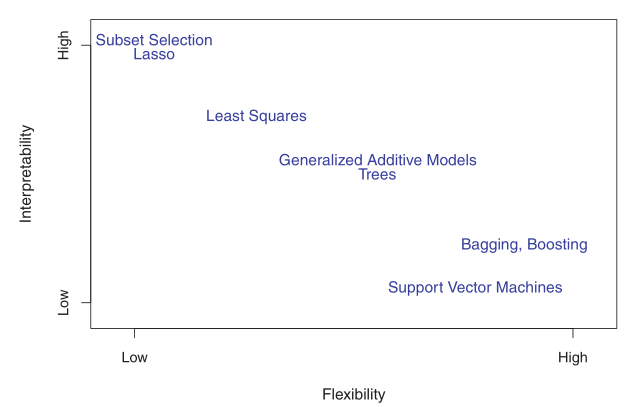
\includegraphics[scale=0.7]{src/StatisticalLearning/Trade-Off_Prediction-Interpretability.PNG}
\caption{A representation of the tradeoff between flexibility and interpretability, using different statistical learning methods. In general, as the flexibility of a method increases, its interpretability decreases.}
\end{figure}

\subsection{Measuring the Quality of Fit}
In the regression setting, the most commonly-used measure is the mean squared error (MSE), given by
\[ \mathrm{MSE} = \frac{1}{n} \sumn (y_i - \hat{f}(x_i))^2  \]
The MSE will be small if the predicted responses are very close to the true responses.

Note that regardless of whether or not overfitting has
occurred, we almost always expect the training MSE to be smaller than
the test MSE because most statistical learning methods either directly or
indirectly seek to minimize the training MSE.

\paragraph{Overfitting}
Overfitting refers specifically
to the case in which a less flexible model would have yielded a smaller
test MSE.

\paragraph{The Bias-Variance Trade-Off}
The equation below tells us that in order to minimize the expected test error,
we need to select a statistical learning method that simultaneously achieves
low variance and low bias. Note that variance is inherently a nonnegative
quantity, and squared bias is also nonnegative. Hence, we see that the
expected test MSE can never lie below Var(?), the irreducible error
\[ \esp{y_0 - \hat{f}(x_0)} \variance{\hat{f(x_0)}} + [ \mathrm{Bias}(\hat{f}(x_0))]^2 + \variance{\varepsilon} \]
\begin{itemize}
    \item \textbf{Variance} refers to the amount by which $\hat{f}$ would change if we estimated it using a different training data set.  In general, more flexible statistical methods have higher variance.
    \item \textbf{Bias} refers to the error that is introduced by approximating a real-life problem, which may be extremely complicated, by a much simpler model. Generally, more flexible methods result in less bias.
\end{itemize}

\begin{figure}[!ht]
    \centering
    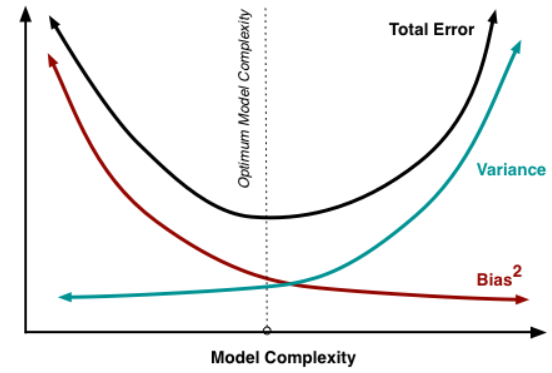
\includegraphics[scale=0.7]{src/StatisticalLearning/Trade-off_Variance-Bias.PNG}
    \caption{Bias-Variance trade-Off}
\end{figure}

\section{Linear Regression}

\subsection{Simple Linear Regression}
\paragraph{Definition}
\[ \hat{y} = \hatbeta_0 + \hatbeta_1 x \]
where the $\hatbeta$ are estimate using the \textbf{least squares} criterion.

\begin{figure}[!ht]
    \centering
    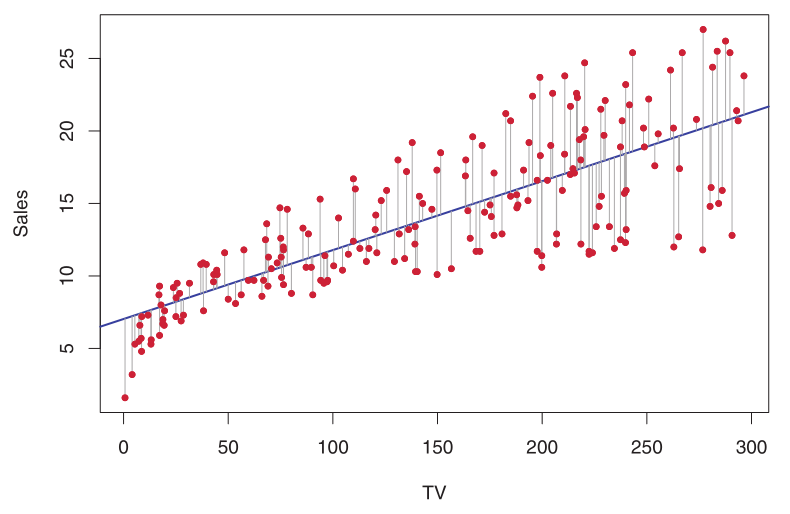
\includegraphics[scale=0.5]{src/StatisticalLearning/SimpleLinearRegression.PNG}
    \caption{Exemple of simple linear regression}
\end{figure}

\paragraph{Residual sum od squares}
We define the residual sum of square as
\[ \mathrm{RSS} = \mathrm{SSE} = \sumn \varepsilon_i = \sumn (y_i - \hat{y}_i)^2 \]

\paragraph{$R^2$ Statistic} 
For simple linear regression, $R^2 = \covar{X, Y}$.

Backward selection cannot be used if p > n, while forward selection can
always be used. Forward selection is a greedy approach, and might include
variables early that later become redundant. Mixed selection can remedy
this.

\section{Multiple Linear Regression}

\subsection{Potential Problems}
When we fit a linear regression model to a particular data set, many prob-
lems may occur. Most common among these are the following:

\paragraph{1. Non-linearity of the Data}
The linear regression model assumes that there is a straight-line relationship between the predictors and the response. If the true relationship is far from linear, then virtually all of the conclusions that we draw from the fit are suspect. In addition, the prediction accuracy of the model can be significantly reduced.

Residual plots are a useful graphical tool for identifying non-linearity. If the residual plot indicates that there are non-linear associations in the data, then a simple approach is to use non-linear transformations of the predictors, such as $\ln(X)$, $\sqrt{X}$, and $X^2$ , in the regression model.

\paragraph{2. Correlation of Error Terms}
An important assumption of the linear regression model is that the error terms, $\varepsilon_1,...,\varepsilon_n$ are uncorrelated. If in fact there is correlation among the error terms, then the estimated standard errors will tend to underestimate the true standard errors.

\begin{figure}[!ht]
    \centering
    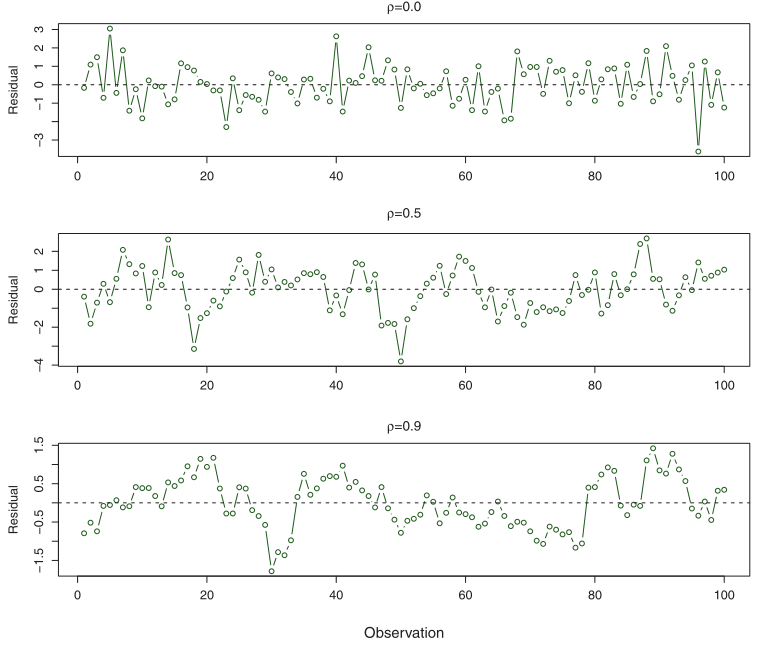
\includegraphics[scale=0.6]{src/StatisticalLearning/CorrelationInErrorTerms.PNG}
    \caption{Plots of residuals time series data sets with differing levels of correlation $\rho$ between error terms for adjacent time points. The graphs on top is good for linear regression}
\end{figure}

\paragraph{3. Non-constant Variance of Error Terms}
Another important assumption of the linear regression model is that the
error terms have a constant variance, $\variance{\varepsilon} = \sigma^2$. If not, we can recognize \textbf{heteroscedasticity} with a funnel shape in the residual plot.

\begin{figure}[!ht]
    \centering
    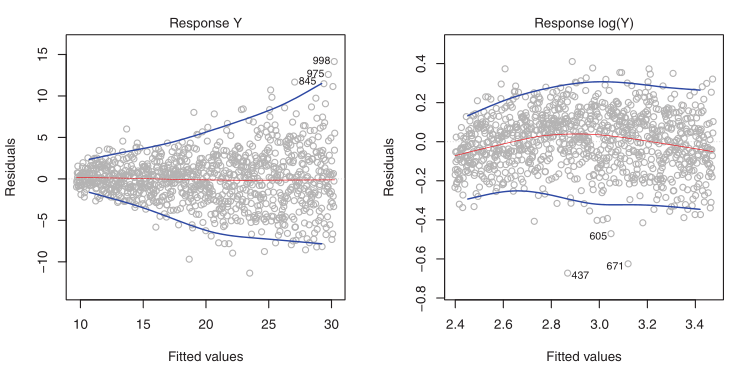
\includegraphics[scale=0.6]{src/StatisticalLearning/Heteroscedasticity.PNG}
    \caption{Residual plots. Left: The funnel shape indicates heteroscedasticity. Right: The predictor has been log-transformed, and there is now no evidence of heteroscedasticity.}
\end{figure}

 When faced with this problem, one possible solution is to transform the response Y using a concave function such as $\ln(Y)$ or $\sqrt{Y}$. Such a transformation results in a greater amount of shrinkage of the larger responses, leading to a reduction in heteroscedasticity. Sometimes, we can also use \textbf{weighted least squares}.

\paragraph{4. Outliers}
An outlier is a point for which $y_i$ is far from the value predicted by the model. Outliers can arise for a variety of reasons, such as incorrect recording of an observation during data collection.

\begin{figure}[!ht]
    \centering
    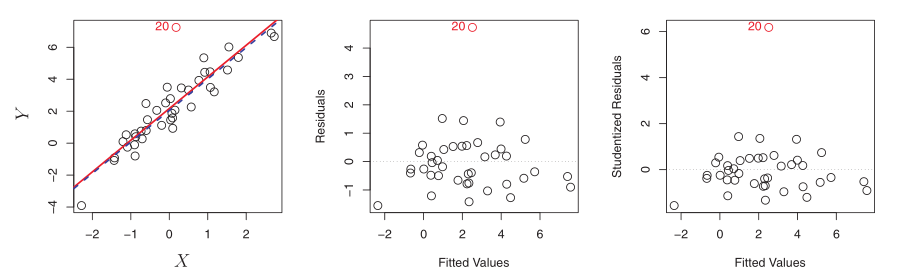
\includegraphics[scale=0.6]{src/StatisticalLearning/Outlier.PNG}
    \caption{Center: The residual plot clearly identifies the outlier. Right: The outlier has a studentized residual of 6; typically we expect values between -3 and 3.}
\end{figure}

Outlier can affect our MSE estimation, resolving in inadequate $R^2$ or confidence interval. We can remove the outlier to resolve this issue.

\paragraph{5. High Leverage Points}
In constrast of \emph{outlier} that are unusual $y_i$, leverage are unusual value of $x_i$. 

\begin{figure}[!ht]
    \centering
    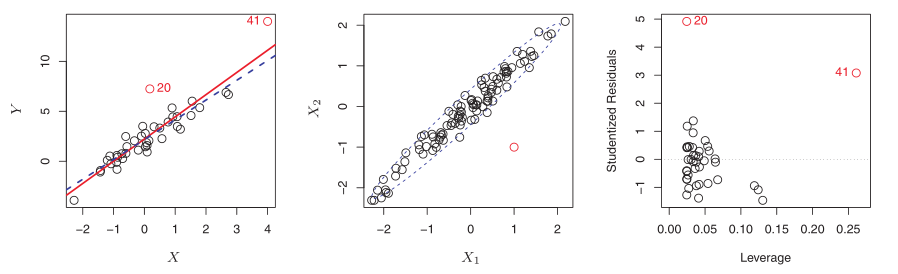
\includegraphics[scale=0.6]{src/StatisticalLearning/Leverage.PNG}
    \caption{Left: Observation 41 is a high leverage point, while 20 is not. The red line is the fit to all the data, and the blue line is the fit with observation 41 removed. Center: The red observation is not unusual in terms of its $X_1$ value or its $X_2$ value, but still falls outside the bulk of the data, and hence has high leverage. Right: Observation 41 has a high leverage and a high residual.}
\end{figure}

For simple linear regression, we can compute the leverage statistic define as
\[ h_i = \frac{1}{n} + \frac{(x_i - \bar{x})^2}{\sum (x_i - \bar{x})^2} \]
where $\frac{1}{n} < h_i < 1$ and $\sum h_i = \frac{(p+1)}{n}$.
So if a given observation has a leverage statistic that greatly exceeds $(p+1)/n$, hen we may suspect that the corresponding point has high leverage.

\paragraph{6. Collinearity}
Collinearity refers to the situation in which two or more predictor variables collinearity are closely related to one another.

\begin{figure}[!ht]
    \centering
    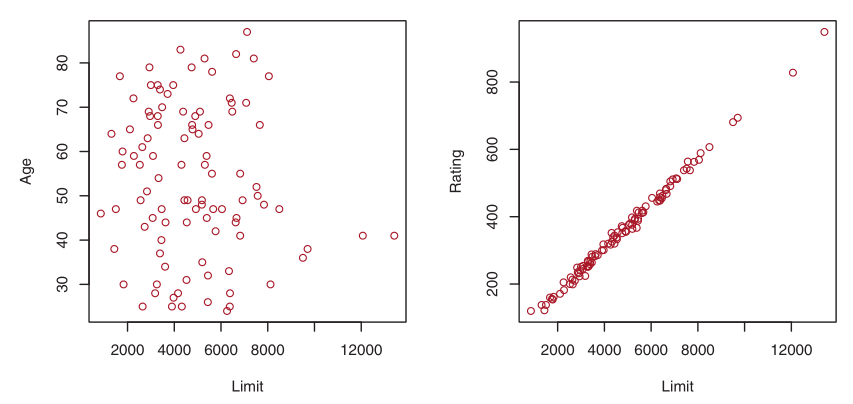
\includegraphics[scale=0.6]{src/StatisticalLearning/Collinearity.PNG}
    \caption{Left: A plot of age versus limit. These two variables are not collinear. Right: A plot of rating versus limit. There is high collinearity.}
\end{figure}

The presence of collinearity can pose problems in the regression context, since it can be difficult to separate out the individual effects of collinear variables on the response.

\section{Classification}
\subsection{Logistic Regression}
In logistic regression, we use the logistic function to be sure that the probability of success given you are in group $i$, $\pi$, is between 0 and 1.
\[ \pi = \frac{e^\eta}{1 + e^\eta} \]
where $\eta = \hatbeta_0 + ... + \hatbeta_p X_p$.

\paragraph{Estimating the Regression Coefficients}
To fit the model, we use the \textbf{maximum likelihood} method. In the case of simple linear models, we can compute the estimation with
\[ \mathcal{L}(\beta_0, \beta_1) = \prod_{i:y_i=1} \pi_i \prod_{i:y_i=0} (1 - \pi_i) \]
\newpage

\begin{figure}[!ht]
    \centering
    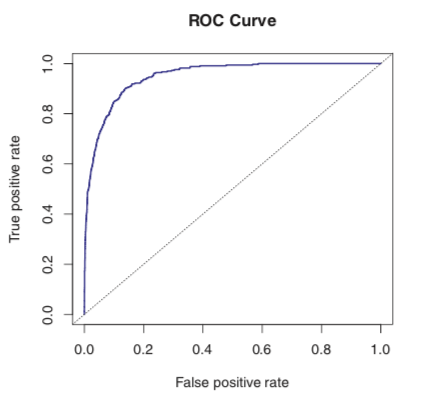
\includegraphics[scale=0.7]{src/StatisticalLearning/ROC-Curve.png}
    \caption{ROC curve used to see the fit of a binomial model. We want to maximize the true rate and minimize the false rate. We want the graph to be as much as possible in the top-left corner of the graph.}
\end{figure}


\paragraph{Cross-Validation on Classification Problems}
Cross-validation works just as described earlier in this chapter, except that rather than using MSE to quantify test error, we instead use the number of misclassified observations.
\[ \mathrm{CV}_{(n)} = \frac{1}{n} \sumn \mathrm{Err}_i\]
where $\mathrm{Err}_i = \indic{y_i \neq \hat{y}_i}$.

\section{Resampling Methods}
The process of evaluating a model’s performance is known as model assessment, whereas the process of selecting the proper level of flexibility for a model is known as model selection.

\subsection{Linear Model Selection and Regularization}
We discuss in this chapter some ways in which the simple linear model can be improved with better prediction accuracy and model interpretability. We achieve this by replacing plain least squares fitting with some alternative fitting procedures

\begin{itemize}
    \item \textbf{Prediction Accuracy} If n is not much larger than $p$, then there can be a lot of variability in the least squares fit, resulting in overfitting and consequently poor predictions on future observations not used in model training. And if p > n, then there is no longer a unique least squares coefficient estimate: the variance is infinite so the method cannot be used at all. By constraining or shrinking the estimated coefficients, we can often substantially reduce the variance at the cost of a negligible increase in bias.
    \item \textbf{Interpretability}  It is often the case that some or many of the variables used in a multiple regression model are in fact not associated with the response. Including such irrelevant variables leads to unnecessary complexity in the resulting model. By removing these variables we can obtain a model that is more easily interpreted.
\end{itemize}


There are many alternatives, both classical and modern, to using least squares to fit:
\begin{itemize}
    \item Subset Selection. 
    \item Shrinkage.
    \item Dimension Reduction. 
\end{itemize}

\subsection{Subset Selection}
\paragraph{Best Subset Selection}
In general, there are 2p models that involve subsets of p predictors.
\begin{figure}[!ht]
    \centering
    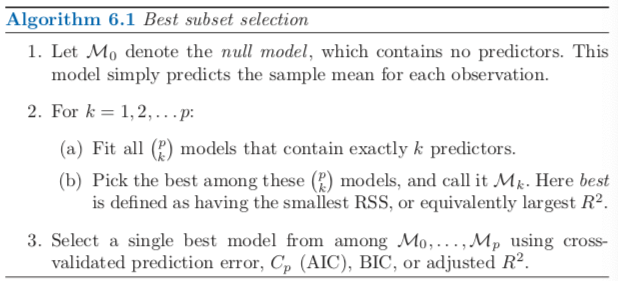
\includegraphics[scale=0.6]{SRC/StatisticalLearning/BestSubsetSelection.png}
\end{figure}

We need to be careful because SSE of these $p + 1$ models decreases monotonically, and the R2 increases monotonically, as the number of features included in the models increases.
Consequently, best sub- set selection becomes computationally infeasible for values of p greater than around 40

\paragraph{Forward Stepwise Selection}

Forward stepwise selection begins with a model containing no predictors, and then adds predictors to the model, one-at-a-time, until all of the predictors are in the model.
\begin{figure}[!ht]
    \centering
    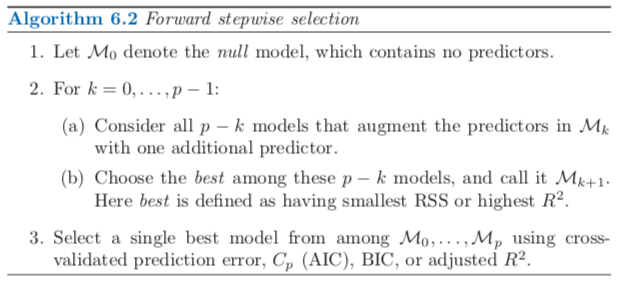
\includegraphics[scale=0.6]{SRC/StatisticalLearning/ForwardStepwiseSelection.png}
\end{figure}

Forward stepwise selection involves fitting
\[ 1 + \sum_{k=0}^{p-1} (p-k) = 1 + \frac{p(p+1)}{2} \]
Forward stepwise selection can be applied even in the high-dimensional setting where $n<p$, but in this case, it only possible to fit $M_0,..., M_{n-1}$ models.

\paragraph{Backward Stepwise Selection}
Backward stepwise selection begins with the full least squares model containing all p predictors, and then iteratively removes the least useful predictor, one-at-a-time.

\begin{figure}[!ht]
    \centering
    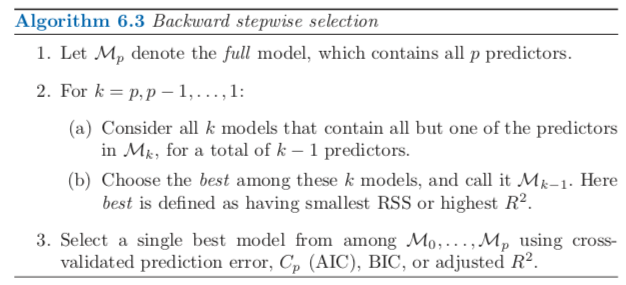
\includegraphics[scale=0.6]{SRC/StatisticalLearning/BackwardStepwiseSelection.png}
\end{figure}


\subsection{Choosing the Optimal Model}
RSS and $R^2$ are not suitable for selecting the best model among a collection of models with different numbers of predictors.

\paragraph{$\mathbf{C_p}$}
For a fitted least squares model containing $d$ predictors, the $C_p$ estimate of \textbf{test MSE} is computed using the equation
\[ C_p = \frac{1}{n} (SSE + 2d\hat{sigma}^2) \]

\paragraph{AIC}
The AIC criterion is defined for a large class of models fit by maximum likelihood.
\[ \mathrm{AIC} = \frac{1}{n\hat{\sigma}^2} (SSE + 2d\hat{\sigma^2}) \]

\paragraph{BIC}
BIC is derived from a Bayesian point of view.
\[ \frac{1}{n} (SSE + \ln(n)d\hat{\sigma^2}) \]
Since $\ln(n) > 2$ for any $n>7$, the BIC give a heavier penalty on models with many variables, and hence results in the selection of smaller models than $C_p$.

\paragraph{Adjusted $\mathbf{R^2}$}
For a least squares model with d variables, the adjusted $R^2$ statistic is calculated as
\[ R_a^2 = 1 - \frac{SSE / (n-d-1)}{SST / (n-1)} \]

\subsection{Shrinkage Methods}
As an alternative of using the least squares to fit a linear model, we can fit a model containing all $p$ predictors using a technique that constrains or regularizes the coefficient estimates. shrinking the coefficient estimates can significantly \textbf{reduce their variance}.

\subsubsection{Ridge Regression}
The ridge regression coefficient estimates $\hatbeta^R$ are the values that minimize.
\[ \sum_{i=1}^{n}\left(y_{i}-\beta_{0}-\sum_{j=1}^{p} \beta_{j} x_{i j}\right)^{2}+\lambda \sum_{j=1}^{p} \beta_{j}^{2}=\mathrm{RSS}+\lambda \sum_{j=1}^{p} \beta_{j}^{2} \]
where $\lambda \geq 0$ is a tunning parameter to be determined separately.

The notation $||\beta||_2$ denotes de $\ell_2$ norm of a vector and is defined as
\[ \sqrt{\sum_{j=1}^n \beta_j^2} \]
It measures the distance of $\beta$ from zero. As $\lambda$ decrease, the $\ell_2$ norm of $\hatbeta_\lambda^R$ will \textbf{always} decrease, and so will $||\hatbeta_\lambda^R||_2/||\hatbeta||_2$. We can see this amount as the amount that the ridge regression coefficient estimates have been shrunken towards zero.
\begin{note}
    \label{note:StandardizedCoefficient}
The standard least squares coefficient estimate are scale invariant: multiplying $X_j$ by a constant $c$ simply leads to a scaling of the least squares coefficient estimates by a factor of $1/c$. In contrast, the ridge regression coefficient estimates can change substantially when multiplying a given predictor by a constant. Therefore, it is best to apply ridge regression after standardizing the predictors, using the formula
    \[ \tilde{x}_{i j}=\frac{x_{i j}}{\sqrt{\frac{1}{n} \sum_{i=1}^{n}\left(x_{i j}-\bar{x}_{j}\right)^{2}}} \]
\end{note}

\paragraph{Why Does Ridge Regression Improve Over Least Squares?}
As $\lambda$ increases, the flexibility of the ridge regression fit decreases, leading to decreased variance but increased bias.

\begin{figure}
    \centering
    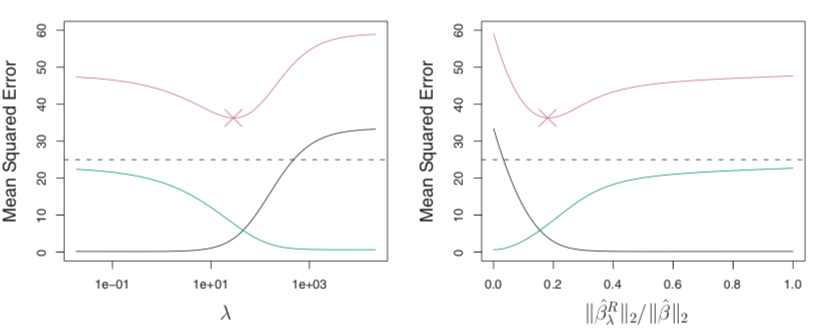
\includegraphics[scale=0.45]{src/StatisticalLearning/Ridge-TradeOff-VarianceBias.png}
    \caption{Squared bias (black), variance (green), and test mean squared error (purple) for the ridge regression predictions. The horizontal dashed lines indicate the minimum possible MSE. The purple crosses indicate the ridge regression models for which the MSE is smallest.}
\end{figure}

\subsubsection{Lasso Regression}
The advantage of Lasso is that the $\hatbeta$ can equal zero, while ridge will include all $p$ parameters.
The Lasso regression minimize
\[ \sum_{i=1}^{n}\left(y_{i}-\beta_{0}-\sum_{j=1}^{p} \beta_{j} x_{i j}\right)^{2}+\lambda \sum_{j=1}^{p}\left|\beta_{j}\right|=\mathrm{RSS}+\lambda \sum_{j=1}^{p}\left|\beta_{j}\right| \]
where $\lambda \geq 0$ is a tunning parameter to be determined separately. The notation $||\beta||_1$ denotes de $\ell_1$ norm of a vector and is defined as
\[ ||\beta||_1 = \sum |\beta_j| \]

\subsubsection{Another Formulation for Ridge Regression and the Lasso}
One can show that the lasso and ridge regression coefficient estimates solve the problems
\[ \underset{\beta}{\operatorname{minimize}}\left\{\sum_{i=1}^{n}\left(y_{i}-\beta_{0}-\sum_{j=1}^{p} \beta_{j} x_{i j}\right)^{2}\right\} \quad \text { subject to } \sum_{j=1}^{p}\left|\beta_{j}\right| \leq s \]
and 
\[ \underset{\beta}{\operatorname{minimize}}\left\{\sum_{i=1}^{n}\left(y_{i}-\beta_{0}-\sum_{j=1}^{p} \beta_{j} x_{i j}\right)^{2}\right\} \quad \text { subject to } \sum_{j=1}^{p}\beta_{j}^2 \leq s \]
If $s$ is small, the estimate of $hatbeta$ will goes tzero. In contrast, if $s$ is large enough that the least squares solution falls within the budget, then the least squares estimate will be generated. 


\subsubsection{Ridge versus Lasso}
Neither ridge regression nor the lasso will universally dominate the other.
Ridge regression more or less shrinks every dimension of the data by the same proportion, whereas the lasso more or less shrinks all coefficients toward zero by a similar amount, and sufficiently small co- efficients are shrunken all the way to zero.
soft- thresholding
\begin{figure}[!ht]
    \centering
    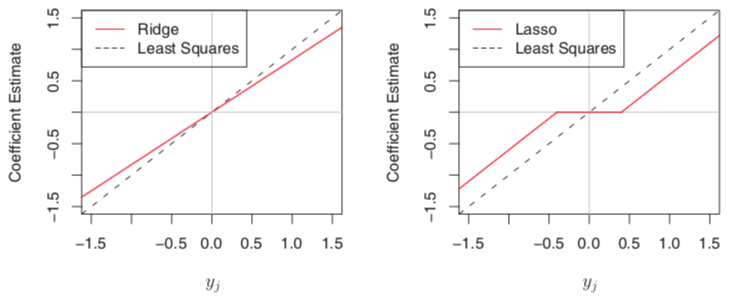
\includegraphics[scale=0.5]{src/StatisticalLearning/Lasso-VS-Ridge.png}
    \caption{Left: The ridge regression coefficient estimates are shrunken proportionally towards zero, relative to the least squares estimates. Right: The lasso coefficient estimates are soft-thresholded towards zero. }
\end{figure}

\subsection{Dimension Reduction Methods}
We now explore a class of approaches that transform the predictors and then fit a least squares model using the transformed variables.

\subsubsection{Definition}
Let $Z_1,...,Z_M$ represent $M<p$ linear combinations of our original $p$ predictor.
\[ Z_m = \sum_{j=1}^p \phi_{jm} X_j \]
for some constants $\phi_{1m},...,\phi_{pm}$. We can then fit the linear regression model
\[ y_i = \theta_0 + \sum_{m=1} \theta_m z_{im} + \varepsilon \quad i=i,...,n \]
using least squares.
\begin{note}
    \[ \sum_{m=1}^{M} \theta_{m} z_{i m}=\sum_{m=1}^{M} \theta_{m} \sum_{j=1}^{p} \phi_{j m} x_{i j}=\sum_{j=1}^{p} \sum_{m=1}^{M} \theta_{m} \phi_{j m} x_{i j}=\sum_{j=1}^{p} \beta_{j} x_{i j} \]
    where 
    \[ \beta_{j}=\sum_{m=1}^{M} \theta_{m} \phi_{j m} \]
\end{note}
This constraint on the form of the coefficients has the potential to bias the coefficient estimates. However, in situations where $p$ is large relative to $n$, selecting a value of $M << p$ can significantly reduce the variance of the fitted coefficients.

\subsubsection{Principal Components Analysis}
We want to combine $p$ variables into only one $Z_1$, that will capture the maximum of the \textbf{variability}. The first \textbf{component score} for the observation $i$ is given by 
\[ z_{1,i} = \phi_{11}(x_1 - \bar{x}_2)  + \phi_{12}(x_2 - \bar{x}_2) \]
under the constraint that the norm of the \textbf{component loading} equal unity
\[ \phi_{i,1}^2 + \phi_{i, 2}^2 = 1 \]

The second principal component $Z_2$ is a linear combination of the variables that is uncorrelated with $Z_2$, and has largest variance subject to this constraint. Since $Z_1$ and $Z_2$ are orthogonal, the following equation must be true
\[ \phi_{11}\phi_{12} + \phi_{21}\phi_{22} = 0 \]

\begin{note}
    Even though PCR provides a simple way to perform regression using $M < p$ predictors, it is not a feature selection method.
    In fact, one can show that PCR and ridge regression are very closely related.
\end{note}
\paragraph{Choosing the number of M parameters} In PCR, the number of principal components, M, is typically chosen by cross-validation.

\paragraph{Standardized Predictor} When performing PCR, we generally recommend \hyperref[note:StandardizedCoefficient]{standardizing each predictor}. In the absence of standardization, the high-variance variables will tend to play a larger role in the principal components obtained, and the scale on which the variables are measured will ultimately have an effect on the final PCR model.

\begin{figure}[!ht]
    \centering
    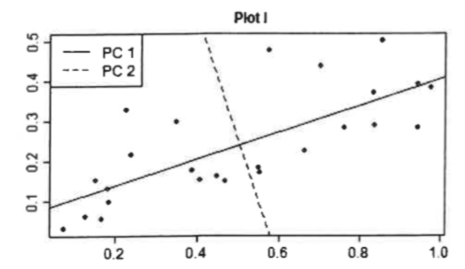
\includegraphics[scale=0.7]{src/StatisticalLearning/PCA.png}
    \caption{Illustration of the first two principal components}
\end{figure}

\subsubsection{Partial Least Squares}
PCA was a unsupervised method of reducing dimension. Partial least square is a supervised method because it the response $Y$ is involve. Roughly speaking, the PLS approach attempts to find directions that help explain both the response and the predictors.

\paragraph{Finding the First Direction}After standardizing the p predictors, PLS computes the first direction $Z_1$ by setting each $\phi_{j1}$ equal to the coefficient from simple linear regression of $Y$ in function of $X_j$. Hence, in computing $Z_1 = \sum_{j=1}^p \phi_{j,1}X_j$, PLS places the highest weight on the variables that are most strongly related to the response.

\paragraph{Finding the Second Direction} To identify the second PLS direction we first adjust each of the variables for $Z_1$, by regressing each variable on $Z_1$ and taking residuals. These residuals can be interpreted as the remaining information that has not been explained by the first PLS direction. We then compute $Z_2$ using this orthogonalized data in exactly the same fashion as $Z_1$ was computed based on the original data.

\section{Moving Beyond Linearity}
Linear model have advantage over other approaches in terms of interpretation and inference. However, their have significant limitations in terms of predic- tive power.

\subsection{Polynomial Regression}
A polynomial regression is define as
\[ y_{i}=\beta_{0}+\beta_{1} x_{i}+\beta_{2} x_{i}^{2}+\beta_{3} x_{i}^{3}+\ldots+\beta_{d} x_{i}^{d}+\varepsilon_{i} \]
where $\beta$ can be estimated using least squares. 
\begin{note}
    We usually don't use d greater than 3 or 4 because otherwise the model can become over flexible and take strange shapes near boundary of the $X$ variable.
\end{note}

\subsection{Step Functions}
To create a step function model we create cutpoints $c_1,...,c_k$ in the range of $X$, and then construct $K+1$ new dummy variable.
\begin{align*}
    c_0(X) &= \indic{X < c_1} \\
    c_1(X) &= \indic{c_1 \leq X < c_2} \\
    c_2(X) &= \indic{c_2 \leq X < c_3} \\
    &\vdots \\
    c_{K-1}(X) &= \indic{c_{K-1} \leq X < c_K} \\
    c_K(X) &= \indic{c_K \leq X}  
\end{align*}
We can then define a step functions model is define as
\[ y_{i}=\beta_{0}+\beta_{1} C_{1}\left(x_{i}\right)+\beta_{2} C_{2}\left(x_{i}\right)+\ldots+\beta_{K} C_{K}\left(x_{i}\right)+\varepsilon_{i} \]
where $C_i(X)$ are dummy variable.

\subsection{Piecewise Polynomials} 
Instead of fitting a high-degree polynomial over the entire range of $X$, piecewise polynomial regression involves fitting separate low-degree polynomials over different regions of $X$.
\paragraph{Example} A piecewise cubic polynomial with a single knot at a point c takes the form
\[ y_{i}=\left\{\begin{array}{ll}{\beta_{01}+\beta_{11} x_{i}+\beta_{21} x_{i}^{2}+\beta_{31} x_{i}^{3}+\epsilon_{i}} & {\text { if } x_{i}<c} \\ {\beta_{02}+\beta_{12} x_{i}+\beta_{22} x_{i}^{2}+\beta_{32} x_{i}^{3}+\epsilon_{i}} & {\text { if } x_{i} \geq c}\end{array}\right. \]
In general, if we place K different knots throughout the range of X, then we will end up fitting K + 1 different cubic polynomials.
In fact, our piecewise constant functions (step function) are piecewise polynomials of degree 0!

\subsection{Spline Model}
\label{subsec:SplineModel}
We define a $d$ spline with $K$ knots as
\[ y_{i}=\beta_{0}+\beta_{1} X + ... + \beta_{d}X^d+\beta_{d+1} h(X, \zeta_1) + ... + \beta_{d+K}h(X, \zeta_K) + \varepsilon\]
where
\[ h(x, \xi)=(x-\xi)_{+}^{3}=\left\{\begin{array}{cl}{(x-\xi)^{3}} & {\text { if } x>\xi} \\ {0} & {\text { otherwise }}\end{array}\right. \]
Then, a spline model have  $1 + d + K$ degrees of freedom.
Unfortunately, splines can have high variance at the outer range of the predictors

\begin{figure}[!ht]
    \centering
    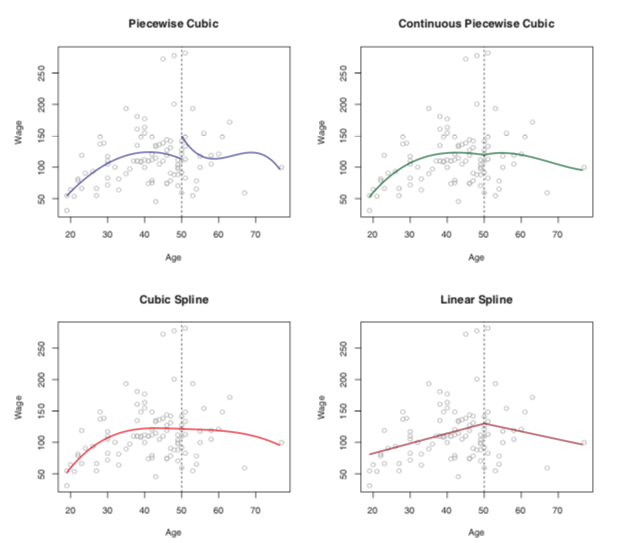
\includegraphics[scale=0.6]{src/StatisticalLearning/NonLinearModelComparaison.png}
    \caption{Four different model fit in the same data}
\end{figure}

\subsubsection{Natural Spline}
A natural spline is a regression spline with additional boundary constraints: the function is required to be linear at the boundary (in the region where X is smaller than the smallest knot, or larger than the largest knot). The number of df is then reduce by $4$ in the case of natural spline $(1 + d + K - 4)$.

\paragraph{Choosing the Location of the Knots}
The regression spline is most flexible in regions that contain a lot of knots, because in those regions the polynomial coefficients can change rapidly. Hence, one option is to place more knots in places where we feel the function might vary most rapidly, and to place fewer knots where it seems more stable. While this option can work well, in practice it is common to place knots in a uniform fashion.

\paragraph{Choosing the Number of Knots}
We also use cross-validation to select the best degree of freedoms.

\subsection{Smoothing Splines}
The function g that minimizes the equation below is known as a smoothing spline.
\[ \sum_{i=1}^{n}\left(y_{i}-g\left(x_{i}\right)\right)^{2}+\lambda \int g^{\prime \prime}(t)^{2} d t \]
where $\lambda$ is a nonnegative tuning parameter. The penalty $\lambda \int g''(t)^2dt$ encourages $g(x)$ to be smooth. The larger the value of $\lambda$, the smoother $g(x)$ will be. When $\lambda = 0$, then the penalty term will have no effect, and so the function $g(x)$ will be very jumpy and will exactly interpolate the training observation. When $\lambda \to \infty$, $g(x)$ will be perfectly smooth (i.e. a linear least squares line). 
\begin{note}
    The function $g(x)$ that result from the equation above is a \textbf{natural cubic spline with knots at} $x_1,...,x_n$. However, it is not the same natural cubic spline that one would get if one applied the basis function approach described in \hyperref[subsec:SplineModel]{Spline Model section} with knots at $x_1,...,x_n$, rather, it is a shrunken version of such a natural cubic spline, where the value of the tuning parameter $\lambda$ controls the level of shrinkage.
\end{note}
\paragraph{Choosing the Smoothing Parameter $\mathbf{\lambda}$} It is possible to show that as $\lambda$ increases from $0$ to $\infty$, the effective degrees of freedom, which we write $df_\lambda$, decrease from $n$ to $2$.

\subsection{Local Regression}
Local regression is a different approach for fitting flexible non-linear functions, which involves computing the fit at a target point $x_0$ using only the nearby training observations.

\begin{figure}[!ht]
    \centering
    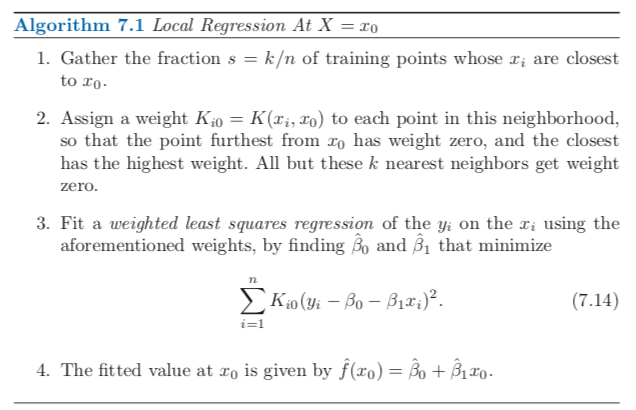
\includegraphics[scale=0.6]{src/StatisticalLearning/LocalRegression.png}
\end{figure}

The smaller the value of s, the more local and wiggly will be our fit; alternatively, a very large value of s will lead to a global fit to the data using all of the training observations.

\subsection{Generalized Additive Models}
In previous section, we present a number of approaches for flexibly predicting a response $Y$ on the basis of a single predictor X. These approaches can be seen as extensions of simple linear regression. Here we explore the problem of flexibly predicting $Y$ on the basis of several predictors, $X_1, ... ,X_P$.
\[ y_i = \beta_0 + f_1(x_{i,1}) + ... + f_p(x_{i,p}) + \varepsilon_i \]
where $f_j(x_{i,j})$ can be any model described in previous section. It is called \textbf{additive} because we calculate a separate $f_j$ for each $X_j$ and then add together all of their contributions.
We can also fit interaction with $f_{i,j}(X_j, X_k)$ with two-dimension model such as local regression.

\paragraph{Advantages}
\begin{itemize}
    \item GAMs allow us to fit a non-linear $f_i$ to each $X_j$, so that we can automatically model non-linear relationships.
    \item The non-linear fits can potentially make more accurate predictions for the response $Y$ .
    \item Because the model is additive, we can still examine the effect of each $X_j$ on $Y$ individually while holding all of the other variables fixed. Hence if we are interested in inference, GAMs provide a useful representation.
    \item The smoothness of the function $f_j$ for the variable $X_j$ can be summarized via degrees of freedom.
\end{itemize}
\paragraph{Disadvantage} 
\begin{itemize}
    \item The main limitation of GAMs is that the model is restricted to be additive. 
\end{itemize}
        

\paragraph{Backfitting} This method fits a model involving multiple predictors by repeatedly updating the fit for each predictor in turn, holding the others fixed. The beauty of this approach is that each time we update a function, we simply apply the fitting method for that variable to a partial residual.

\begin{note}
    A partial residual for $X_3$, for exemple, has the form $r_i = y_i - f_1(x_{i,1}) - f_2(x_{i,2})$. If we know $f_1$ and $f_2$, then we can fit $f_3$ by treating this residual as a response in a non-linear regression on $X_3$.
\end{note}


